The original model consists of the following equations.
\begin{align}
    F(\theta) = \begin{cases}
        F_1(\theta) & \text{if } q \cdot \cos(\theta) > 0 \\
        F_2(\theta) & \text{if } q \cdot \cos(\theta) < 0
    \end{cases}
\end{align}
Where $F_1$ is given by the following equation.
\begin{align}
    F_1(\theta) & = \begin{cases}
        \theta + z_{L_+} + z_1 & \text{if } z_{L_+} < z_{L_0} \\
        \theta + z_{L_0} + z_2 & \text{if } z_{L_+} > z_{L_0}
    \end{cases}
\end{align}
And $F_2$ is similarly given by the following equation.
\begin{align}
    F_1(\theta) & = \begin{cases}
        \theta + z_{R_+} + z_3 & \text{if } z_{R_+} < z_{R_0} \\
        \theta + z_{R_0} + z_4 & \text{if } z_{R_+} > z_{R_0}
    \end{cases}
\end{align}
$z_{L_+}, z_{L_0}, z_{R_+},$ and $z_{R_0}$ must satisfy the following equations.
\begin{subequations}
\begin{align}
    (q \cdot \cos(\theta) + \mu \cdot \chi) \cdot e^{\lambda \cdot z_{L_+}}
    & = q \cdot \cos(\theta + z_{L_+} + z_1) + \mu \cdot \chi \\
    (q \cdot \cos(\theta) + \mu \cdot \chi) \cdot e^{\lambda \cdot z_{L_0}}
    & = q \cdot \cos(\theta + z_{L_0} + z_1) - \mu \cdot \chi \\
    (q \cdot \cos(\theta) + \mu \cdot \chi) \cdot e^{\lambda \cdot z_{R_+}}
    & = q \cdot \cos(\theta + z_{R_+} + z_1) + \mu \cdot \chi \\
    (q \cdot \cos(\theta) + \mu \cdot \chi) \cdot e^{\lambda \cdot z_{R_0}}
    & = q \cdot \cos(\theta + z_{R_0} + z_1) - \mu \cdot \chi
\end{align}
\end{subequations}
While $z_1, z_2, z_3,$ and $z_4$ must satisfy these equations.
\begin{subequations}
\begin{align}
    (q \cdot \cos(\theta + z_{L_+}) + \chi + 1) \cdot e^{\lambda \cdot z_1} - 1
    & = q \cdot  \cos(\theta + z_{L_+} + z_1) + \mu \cdot \chi \\
    (q \cdot \cos(\theta + z_{L_0}) + \chi + 1) \cdot e^{\lambda \cdot z_2} + 1
    & = q \cdot  \cos(\theta + z_{L_0} + z_2) - \mu \cdot \chi \\
    (q \cdot \cos(\theta + z_{R_+}) + \chi + 1) \cdot e^{\lambda \cdot z_3} - 1
    & = q \cdot  \cos(\theta + z_{L_+} + z_3) + \mu \cdot \chi \\
    (q \cdot \cos(\theta + z_{R_0}) + \chi + 1) \cdot e^{\lambda \cdot z_4} + 1
    & = q \cdot  \cos(\theta + z_{R_0} + z_4) - \mu \cdot \chi
\end{align}
\end{subequations}

\todo{validate formulas, 2.5b and 2.5c missing $+ z_i$ in cos}

The values for $\chi, \lambda, \mu,$ and $q$ come from the parameters of the model.
The parameters are $\chi_0, E_0, \beta, f, L, R, V_m,$ and $\mu$.
$\mu$ is directly applied in the equations above, while $\chi$ and $q$ consist of multiple parameters.
The values of $\chi$ and $q$ are given by the following equations.
\begin{align}
    \chi & = \dfrac{R \cdot \chi_0}{\beta \cdot E_0} \\
    \lambda & = \dfrac{-R}{L \cdot 2 \cdot \pi \cdot f} \\
    q & = \dfrac{R \cdot V_m}{\beta \cdot E_0}
\end{align}
\todo{stimmt das so?}

We are interested in the dynamics that emerge when fixing the parameters $\beta = 1, f = 150, L = 4.2 \cdot 10^{-3}, R = 2, V_m = 5,$ and $\mu = 0.5$.
The parameters $E_0$ and $\chi_0$ are varied.
$E_0$ is in the range $[14, 28]$, while $\chi_0$ is in the range $[0.1, 0.65]$.
When scanning this parameter plane for the period of emerging cycles, \Cref{fig:yunus.2pi.2d.full} emerges.

\begin{figure}
    \centering
    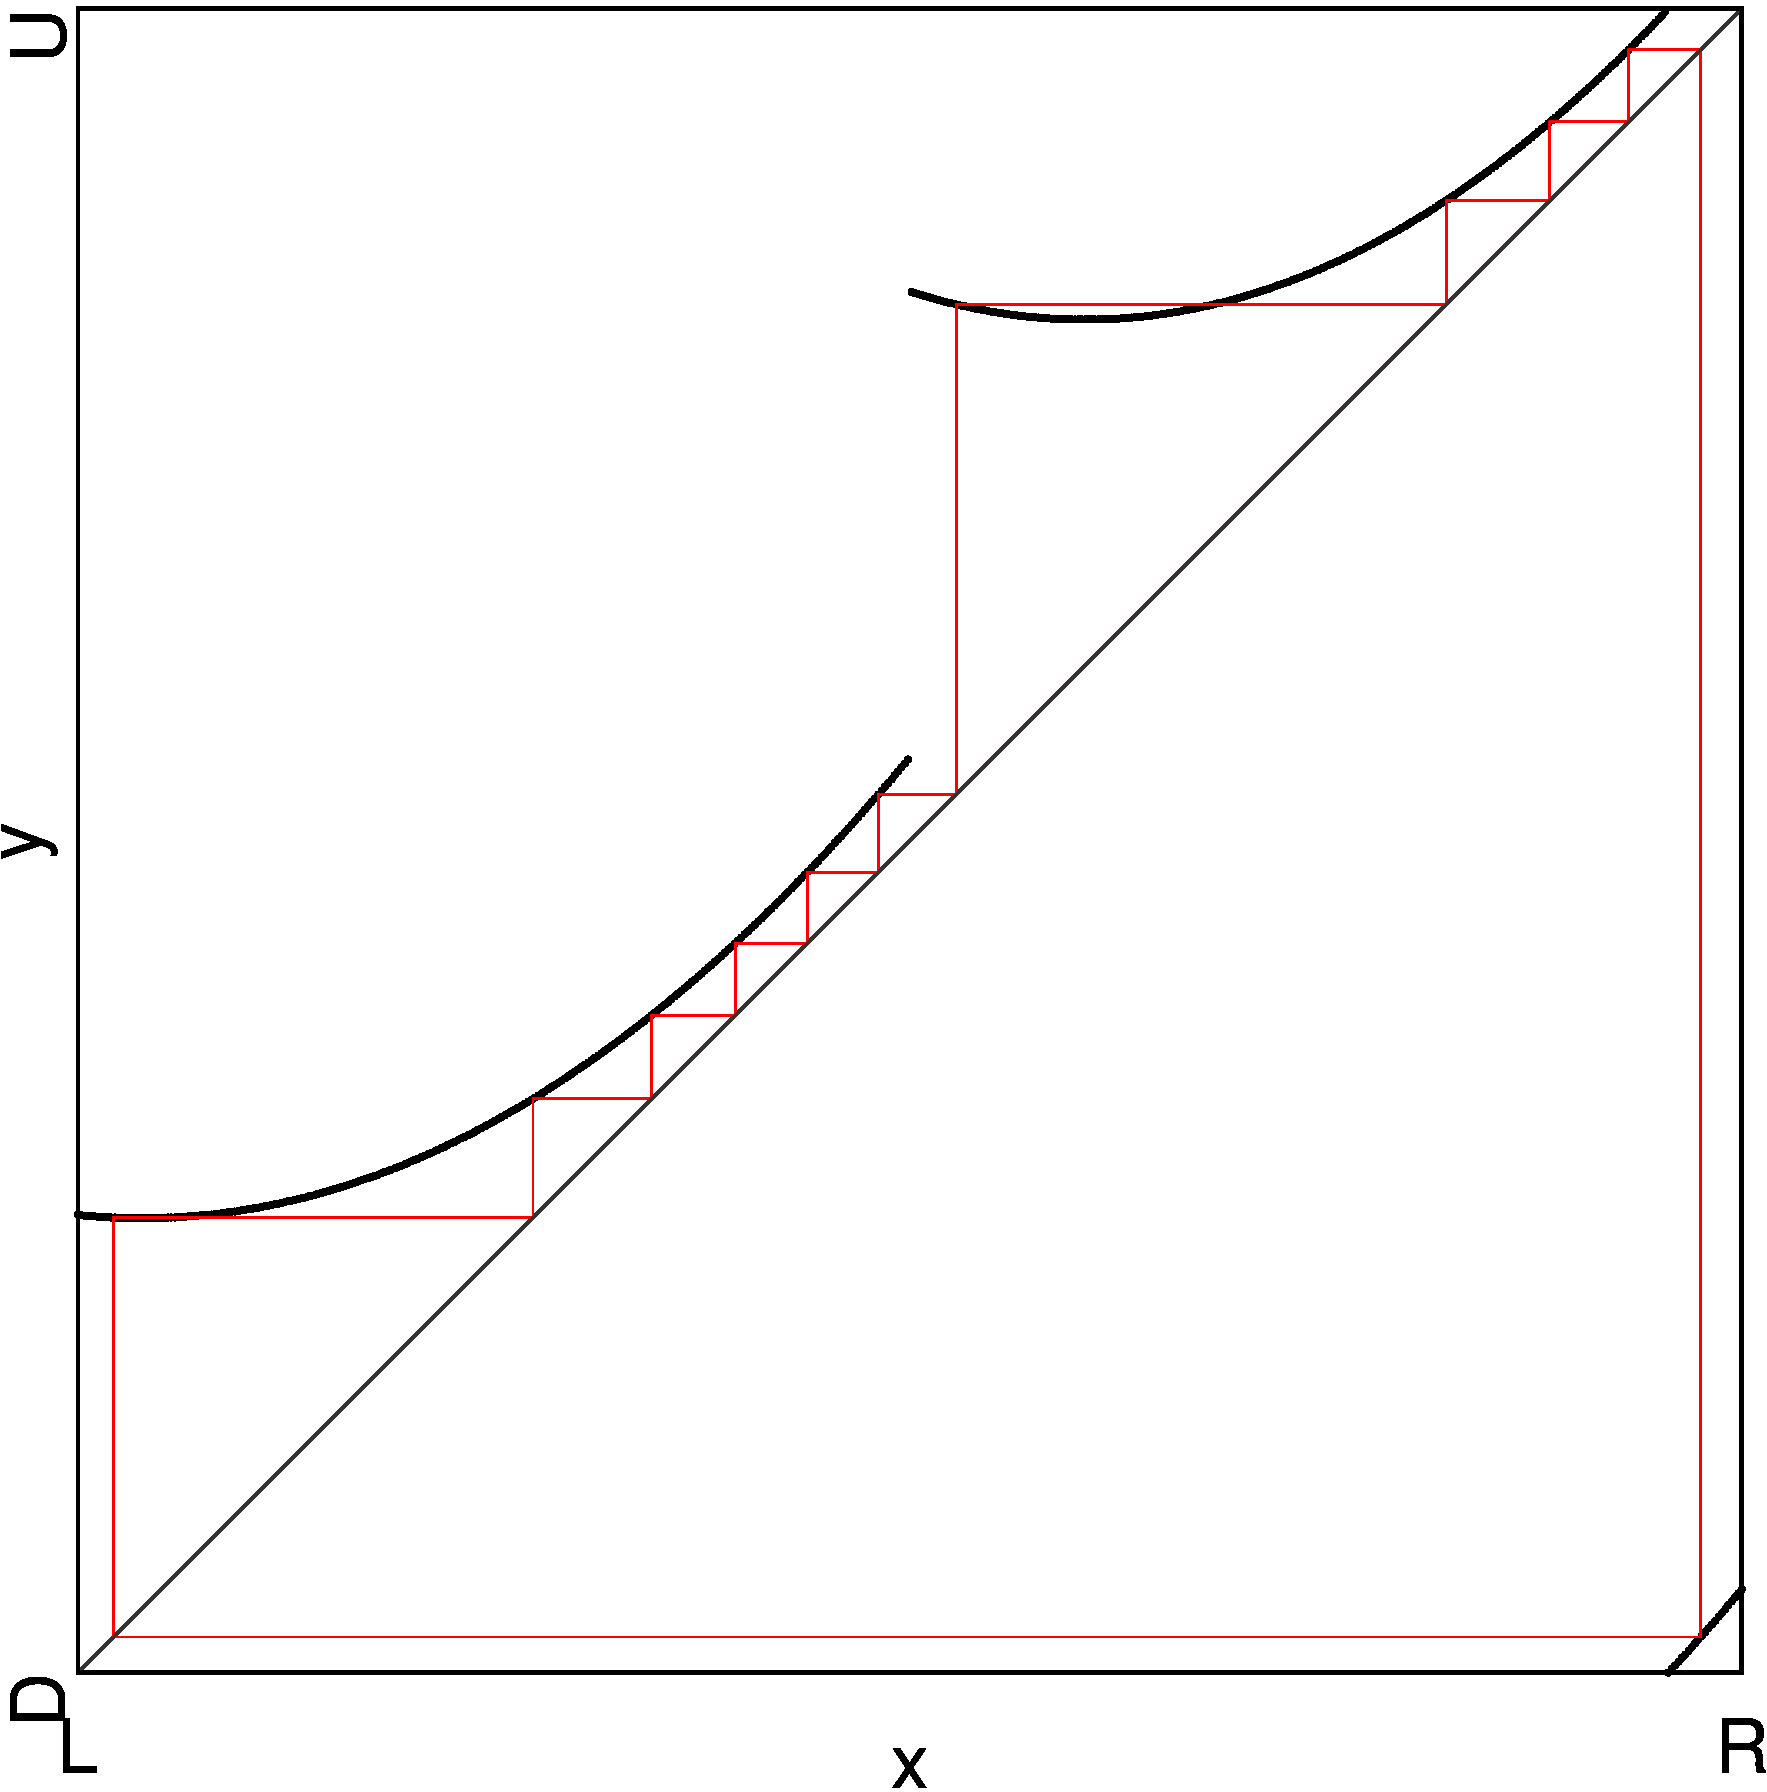
\includegraphics[width=0.6\textwidth]{99_Yunus/2D_Period/result.png}
    \caption{2D Scan of Original Model}
    \label{fig:yunus.2pi.2d.full}
\end{figure}

\todo{cobwebs along red line}
